\section{Theorie}
\label{sec:theorie}

Laser (Light Amplification by Stimulated Emission of Radiation) sind Quellen
elektromagnetischer Strahlung, die kohärentes und monochromatisches Licht mit
hoher Intensität emittieren. Laser bestehen stets aus drei Hauptkomponenten:
Pumpquelle, Resonator und aktives Lasermedium. Im Folgenden sollen die
Funktionsweise eines Lasers sowie die Eigenschaften der Laserstrahlung kurz
erläutert werden:

\begin{figure}[htb]
  \centering
  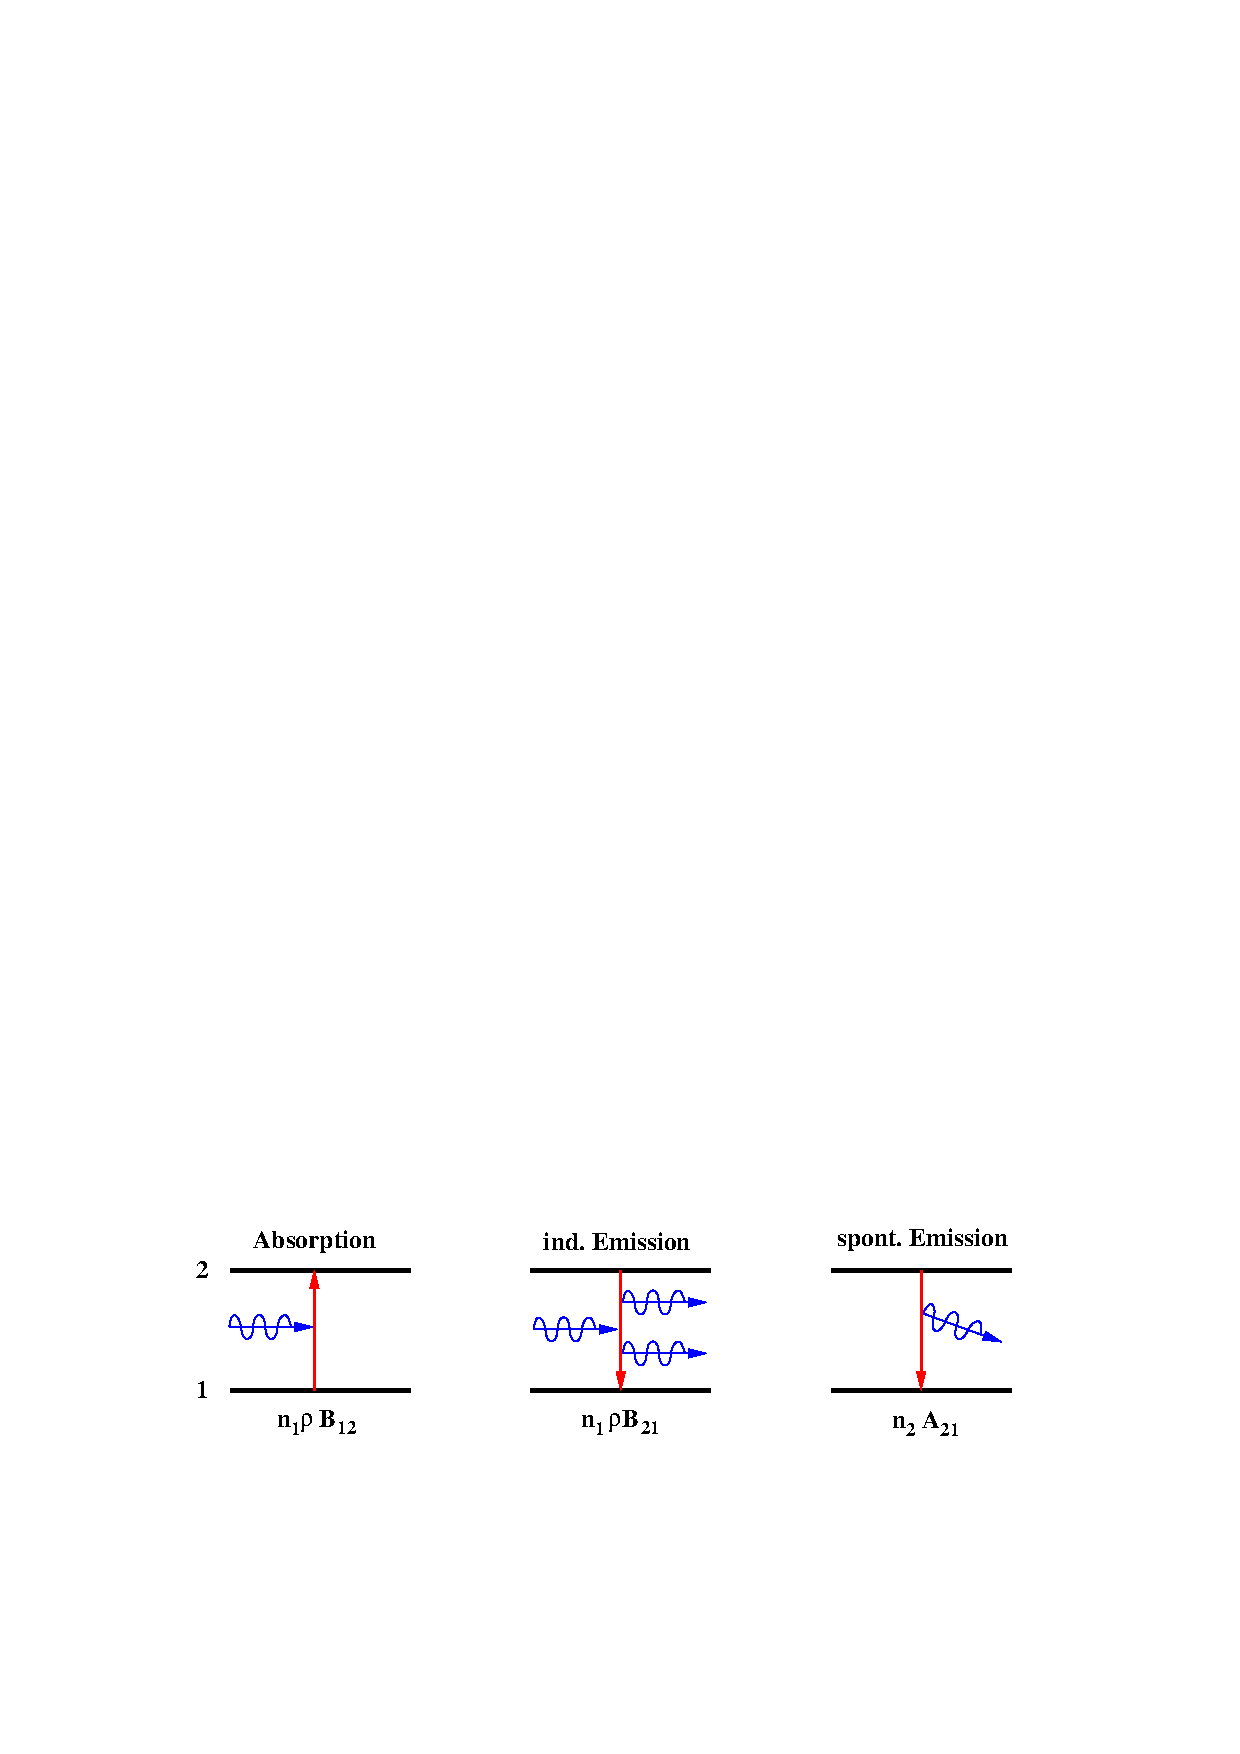
\includegraphics[width=0.9\textwidth]{figures/fig_Übergänge.pdf}
  \caption{Schemata für die Absorption und Emission eines
  Strahlungsfeldes~$\rho(\nu)$ bei einem \num{2}-Niveau-System.}
  \label{fig:Übergänge}
\end{figure}

Das Strahlungsspektrum eines Lasers wird durch die Eigenschaften des aktiven
Lasermediums festgelegt. Ziel ist es, das Lasermedium so zu beeinflussen, dass
durch Wechselwirkung mit dem Strahlungsfeld eine Verstärkung der eingehenden
Strahlung erfolgt. Wesentlich für den Verstärkungsprozess ist die im Folgenden
diskutierte, durch einfallende Photonen ausgelöste induzierte Emission. Zur
Vereinfachung wird ein idealisiertes 2-Niveau-System eines Atoms im Lasermedium
betrachtet. Gemäß der Maxwell-Boltzmann-Verteilung überwiegt im thermischen
Gleichgewicht die Besetzung des Grundzustandes. Durch äußere Anregung, zum
Beispiel in Form von elektrischen Entladungen, werden Elektronen auf ein höheres
Energieniveau gehoben. Tritt nun ein einfallendes Photon in Wechselwirkung mit
dem angeregten Atom, so kann es zu einer induzierten Emission kommen. Dabei wird
ein weiteres Photon derselben Energie, Phase und Ausbreitungsrichtung abgegeben.
Findet dieser Prozess häufig genug statt, so kommt es zu einer kaskadenartigen
Verstärkung der Strahlung. Weitere Wechselwirkungen sind die spontane Emission
eines Photons durch ein angeregtes Elektron, welche nicht durch ein externes
Photon ausgelöst wird, sowie die Absorption eines Photons durch ein Elektron.
Das Verhältnis von Absorption (A), spontaner Emission (E) und induzierter
Emission (IE) ist durch die drei Gleichungen
%
\begin{align}
  \dot{N}_{\mathrm{A}}&=n_1\rho(\nu)B_{12}, \\
  \dot{N}_{\mathrm{IE}}&=n_2\rho(\nu)B_{21} \\
  \shortintertext{und}
  \dot{N}_{\mathrm{E}}&=n_2A_{21}
\end{align}
%
mit den Einsteinkoeffizienten~$A_{21}$, $B_{12}$ und~$B_{21}$ gegeben. $n_1$
und~$n_2$ sind hierbei die Besetzungszahlen für den Grundzustand und den
angeregten Zustand und~$\rho$ die Energiedichte des Strahlungfeldes. $\dot{N}$
ist die Anzahl der Photonen, die pro Volumeneinheit und Sekunde abgegeben oder
aufgenommen werden. Für den Fall, das sich Absorption und Emission vollständig
kompensieren, gilt
%
\begin{align}
  \frac{\mathrm{d}n_1}{\mathrm{d}t}&=-n_1B_{12}\rho+N_2B_{21}\rho+n_2A_{21} \\
  \shortintertext{und}
  \frac{\mathrm{d}n_2}{\mathrm{d}t}&=+N_1B_{12}\rho-n_2B_{21}\rho-n_2A_{21}.
\end{align}

\begin{figure}[htb]
  \centering
  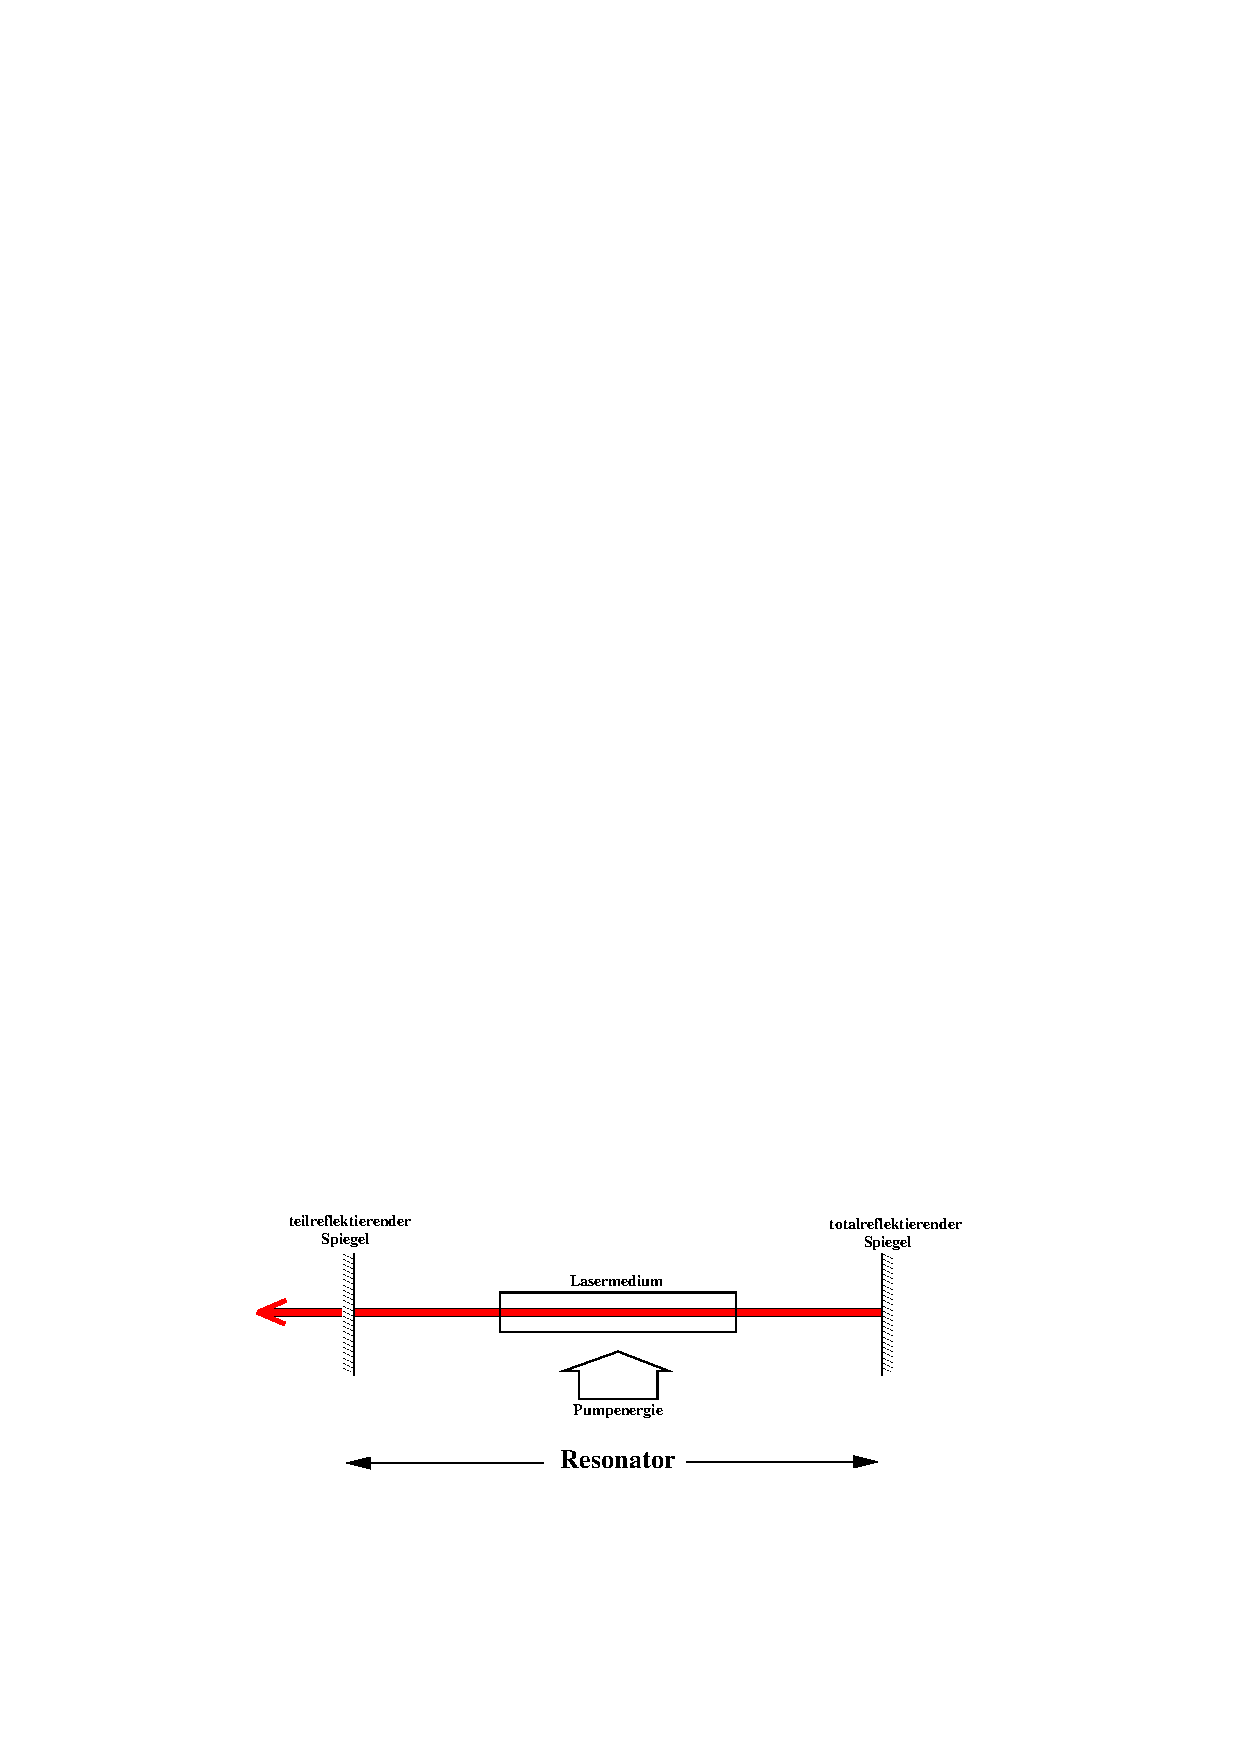
\includegraphics[width=0.9\textwidth]{figures/fig_Resonator.pdf}
  \caption{Prinzipielle Funktionsweise eines Lasers.}
  \label{fig:Resonator}
\end{figure}

Damit die Strahlung hinreichend verstärkt wird, ist es notwendig, dass der
Laserstrahl das Medium mehrmals durchläuft. Dazu ist das Lasermedium innerhalb
eines optischen Resonators positioniert. Der Resonator besteht aus zwei sich
gegenüberstehenden Spiegeln, zwischen denen der Strahl hin und her läuft. Ein
Spiegel ist als sogenannter Auskoppelspiegel realisiert, der für den Strahl
teildurchlässig ist und durch den der Laserstrahl die Apparatur verlassen kann.
Für den stabilen Betrieb muss die Verstärkung durch induzierte Emission des
Strahls größer sein, als die Verluste an den Resonatorspiegeln. Dieses Kriterium
ist erfüllt, wenn die Stabilitätsbedingung
%
\begin{equation}
  0\leq g_1\cdot g_2<1
  \label{eq:bedingung}
\end{equation}
%
gilt. Die hierfür benötigten Parameter sind durch~$g_i=1-L/r_i$ gegeben,
wobei~$r_i$ den Krümmungsradius des jeweiligen Spiegels und~$L$ die Gesamtlänge
des Resonators beschreibt.

Aufgrund der Größe des Resonators erfüllen viele Moden der im Resonator
stehenden Welle die Resonanzbedingung. Angelehnt an die Theorie der Hohlleiter
werden die~$\text{TEM}_{lpq}$-Moden beschrieben durch die Anzahl~$q$ der
Wellenlängen im Resonator, sowie durch die Anzahl~$l$ und~$p$ der Wellenknoten
in der~$x$- und~$y$-Richtung. Für einen konfokalen Resonator mit runden Spiegeln
(Radius~$R$) ergibt sich die Intensitätsverteilung der Strahlung zu
%
\begin{gather}
  I_{lpq}\propto\cos^2(l\varphi)\frac{(2\rho)^4}{(1+Z^2)^{(1+l)}}\left(L_p^q\left(\frac{(2\rho)^2}{1+Z^2}\right)\right)^2\exp\left(-\frac{2\rho^2}{1+Z^2}\right) \\
  \shortintertext{mit}
  \rho=\left(\frac{2\pi}{R\lambda}\right)^{1/2} \\
  \shortintertext{und}
  Z=\left(\frac{2}{R}\right)z.
\end{gather}
%
Die Parameter~$l$ und~$p$ werden als transversale Modenzahl bezeichnet.
Bei~$L_p^q(u)$ handelt es sich um die zugeordneten Laguerre-Polynome.

Im hier durchgeführten Versuch wird ein Helium-Neon-Gaslaser verwendet, der als
Lasermedium ein Gasgemisch aus Helium und Neon in einem Verhältnis von
ungefähr~\num{5} zu~\num{1} bei geringem Druck~$(\approx\SI{133}{\pascal})$
enthält. Die Besetzungsinversion wird durch elektrische Entladungen erreicht.
Das eigentliche Lasermedium ist das Neon. Das Helium dient als Pumpgas, welches
durch die elektrischen Entladungen angeregt wird und Energie an die Neon-Atome
durch Stöße zweiter Art abgibt. Helium-Neon-Laser arbeiten typischerweise bei
einer Wellenlänge von~$\lambda=\SI{632.8}{\nano\metre}$.
